\subsection{Solver loop}

Here we quickly describe the implementations provided for each step of the algorithm.
Most of the details are explained in Section~\ref{sec:algorithm}.


\subsubsection{\texttt{RateContainer} classes}

\begin{figure}[!h]
  \centering
  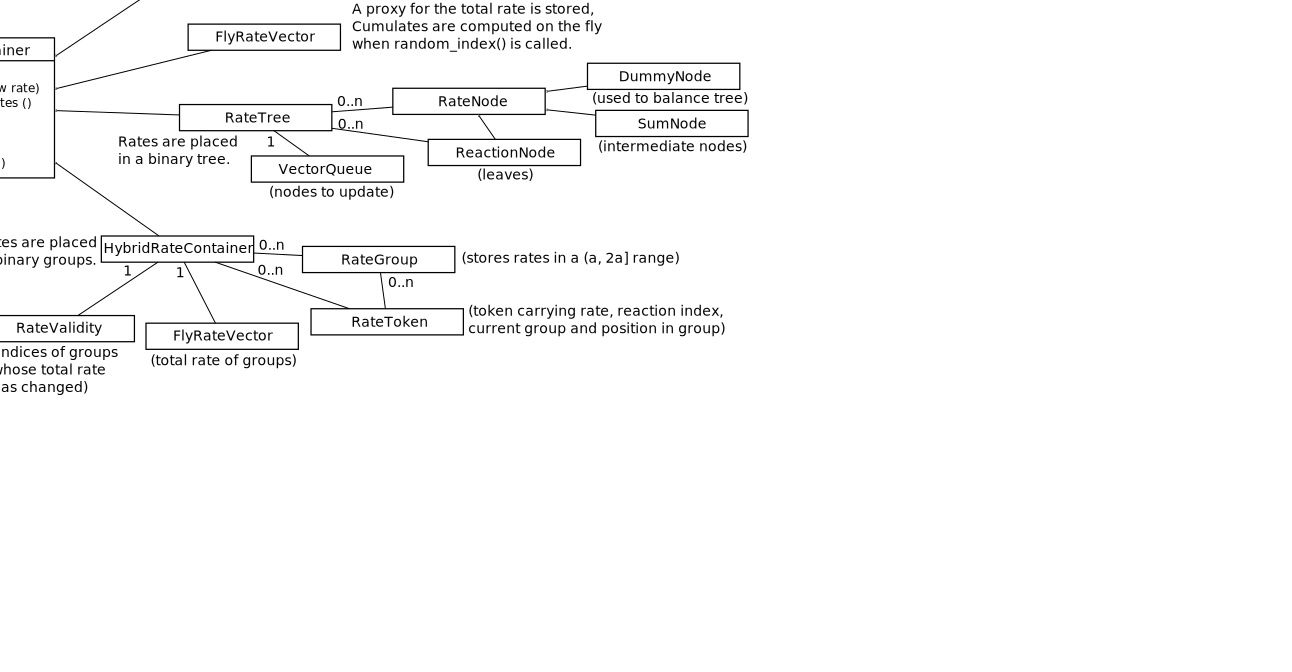
\includegraphics[width=\linewidth]{rate_container}
  \caption{
  Implementations provided to store rates and perform a multinomial drawing.
  Implicitly, all theses classes use \texttt{RandomHandler} to perform their random drawings.
  }
\label{fig:rate_container}
\end{figure}

We start with the lowest level classes,
which perform one of the central tasks of the Gillespie algorithm:
drawing a reaction from reaction rates.
For efficiency reasons, we propose several implementation of the algorithm~\reffigp{fig:rate_container}.
Comparison and description of theses classes are given in Section~\ref{sec:algorithm}.

Note that multinomial drawing occurs within the solver loop,
but also within some reactions such as \texttt{Loading} or \texttt{SequenceBinding},
so these classes are used quite extensively throughout the simulation.


\subsubsection{\texttt{RateManager} classes}

\begin{figure}[!h]
  \centering
  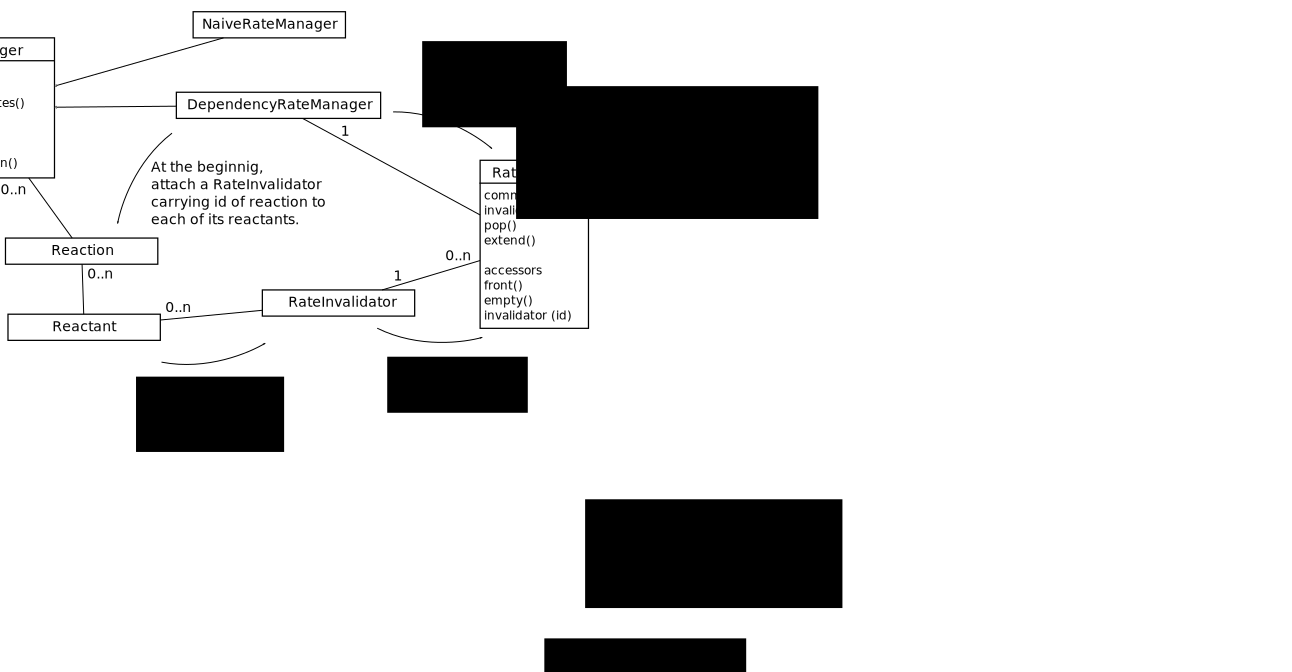
\includegraphics[width=\linewidth]{rate_manager}
  \caption{
  Implementations provided to update reaction rates.
  Note that the drawing part of the algorithm is always delegated to a \texttt{RateContainer}.
  \texttt{DependencyRateManager} uses an Observer pattern to monitor which rates have changed.
  }
\label{fig:rate_manager}
\end{figure}

The second layer of the solver loop ensures that the rates are updated when needed to.
Two implementations are proposed for this task~\reffigp{fig:rate_manager}.
The \texttt{NaiveRateManager} updates every rate.
While it is inefficient, it can be used as a reference to test other managers.
The \texttt{DependencyRateManager} uses an observer pattern to update only reactions
for which a reactant concentration has changed (see Section~\ref{sec:algorithm} for further details).

\subsubsection{\texttt{Solver} classes}

\begin{figure}[!h]
  \centering
  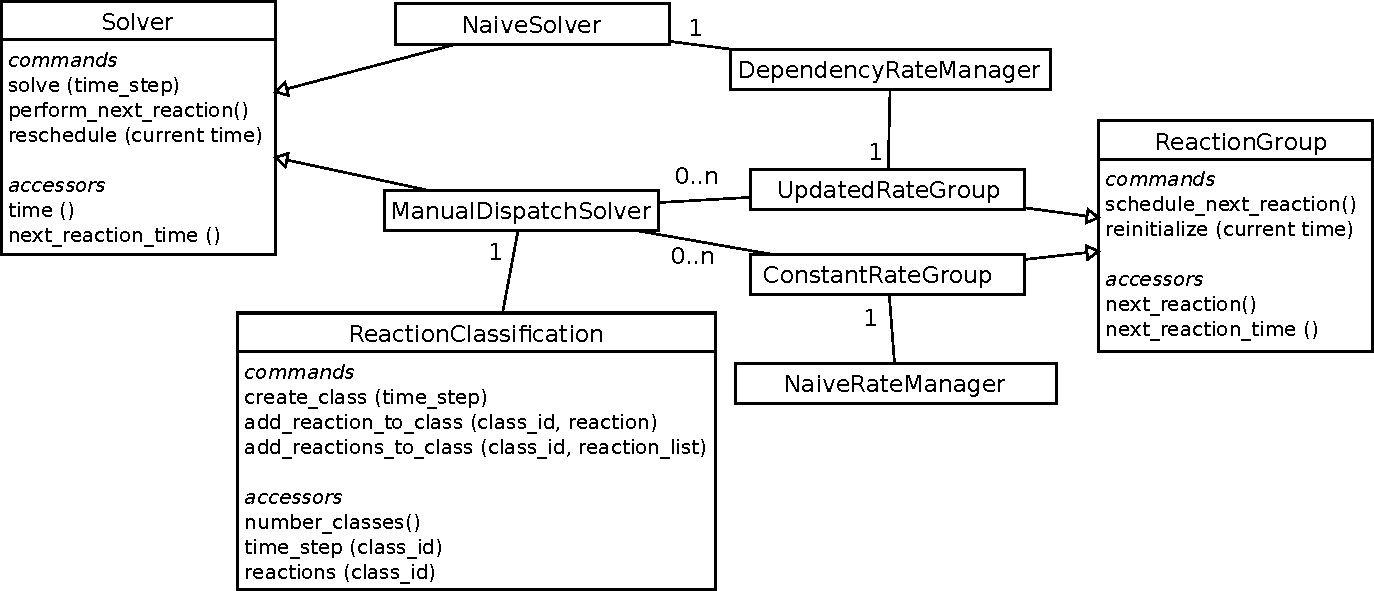
\includegraphics[width=\linewidth]{solver}
  \caption{Two implementations of the \texttt{Solver} class organizing rate updating.
  \texttt{NaiveSolver} forces recomputation of rates at each time step.
  \texttt{ManualDispatchSolver} puts reactions into groups:
  reactions in \texttt{UpdatedRateGroup} are updated after every reaction
  while those in \texttt{ConstantRateGroup} only at user-defined steps defined in \texttt{ReactionClassification}.
  Note that all \texttt{Solver} classes use at least a variant of \texttt{RateManager}
  at some point to delegate storing and updating of rates.}
\label{fig:solver_details}
\end{figure}

For the moment, only one solver class is fully available to the user, \texttt{NaiveSolver},
which implements the exact Gillespie algorithm.
Another variant called \texttt{ManualDispatchSolver} is implemented,
where the user can assign a time step to each reaction at which its rate will be updated~\reffigp{fig:solver_details}.
However, when the rate of a reaction is a constant,
there is a risk that its reactants will run out
and the reaction will be impossible to realize or reactant number will become negative.
In the simulator, the latter case is forbidden, so \texttt{ManualDispatchSolver}
ignores reactions impossible to perform due to reactant unavailability.
